\chapter{Context\label{section:context}}

In this chapter, I will introduce all the concepts needed for the understanding
the design of the adaptations and
the experiments I conducted in this thesis.
I will also give an overview of works related to the topic.

\section{Low Power Wide Area Network (LPWAN)\label{section:lpwan}}

My work is based on the LoRa radio protocol which belongs to the LPWAN network
family.
Sigfox, NB-IoT are other well known LPWAN radio protocols.
The LPWAN network family is typically made for sensor networks that require
very limited throughput.
The next four characteristics are what constitute an LPWAN.

\begin{description}
  \item[Low power]: The network is made of battery-operated
    motes that must run for years without replacement.
  \item[Long range]: Mote should transmit over multiple km without a repeater.
  \item[Low cost devices]: No expensive infrastructure requirement and motes
    operate with simple hardware.
  \item[Limited data rate]: Not suited for data-intensive applications.
\end{description}

To keep the energy consumption of motes as low as possible, LPWAN are typically
based on a star-of-star topology with one or more always-on internet gateways
that listens for incoming messages.
This keeps the radio of the motes off as much as possible where multi-hop routing
would require motes to listen for potentially incoming messages and
relay them.
Using such a scheme, considerably increases the power consumption of each
participant, which goes against the principles of LPWAN.
My work explores a solution based on a different MAC protocol to keep intact the
four characteristics of LPWAN while adding multi-hop routing capability to LoRa.

\paragraph{}

My work is part of a larger context that aims to bring IPv6 over Low-Power
Wireless Personal Area Networks (6LoWPAN) for LoRa.

6LoWPAN is an open standard defined in RFC~6282 by the Internet Engineering
Task Force (IETF).
The idea of 6LoWPAN is to bring IPv6 packet over LPWAN and its limited payload
size with the help of a header compression mechanisms.
6LoWPAN brings native IP communication to LPWAN making the Internet protocols
work on those low power devices.
Each mote of the network can communicate with the Internet by passing its
traffic through an edge router.
Edge routers are special devices that handle the data exchange between the
6LoWPAN network and the internet.

\begin{figure}[H]
  \centering
  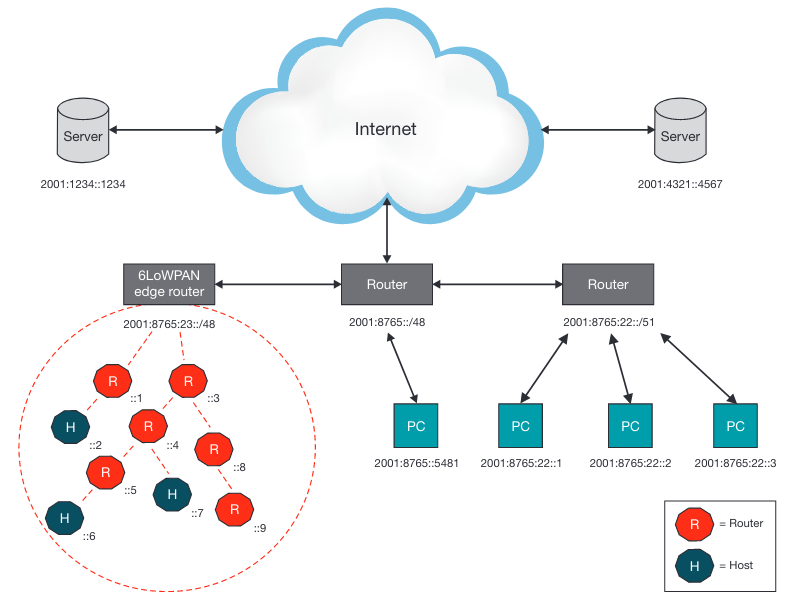
\includegraphics[width=0.8\textwidth]{thesis.tex/chapters/context/fig/6lowpan.png}
  \caption{An example of an IPv6 network with a 6LoWPAN mesh network\cite{olsson20146lowpan}\label{fig:6lowpan}}
\end{figure}

% \paragraph{6TiSCH}
% TODO later in TSCH section
% In the same way as with 6LoWPAN, 6TiSCH defines an adaptation layer for IPv6
% over TSCH named 6top.

\section{LoRa\label{section:lora}}

My work is based around using LoRa Phy, the radio communication protocol.
In this section, I will give an introduction to the protocol and its
modulation parameters.

\paragraph{}

LoRa is a proprietary chirp spread spectrum technology owned by Semtech with
integrated Forward Error Correction (FEC).
LoRa operates in this sub-GHz unlicensed ISM bands. % TODO Cite
The main characteristic of LoRa is that it trades data rates for long-range
transmission and low-power consumption with a maximum data rate of
27 kbps~\cite{8030482}.
LoRa supports bi-directional communications with a maximum payload size of 242
bytes~\cite{loraalliance:lorawanspecification}.

\paragraph{}

This section will cover the LoRa physical layer parameters, the packet
structure and finally, I will explain how all these parameters influence the
Time On Air (ToA).
The physical layer parameters are what constitutes LoRa and these parameters
will be used throughout
chapters~\ref{section:radio}~and~\ref{section:tsch}.
understanding how changes in these parameters will impact LoRa's performance
is important for understanding my work and how LoRa behaves.

\subsection{Chirp Spread Spectrum (CSS) modulation}

LoRa is based on a modified CSS modulation technique.
In telecommunication, modulation techniques are used to transmit information (bits in digital communication like we are using)
by varying the properties of a waveform (e.g. its frequency, phase or amplitude).
Chirp Spread Spectrum modulation, which LoRa is based on, transmits information
by using sinusoidal signals that increase (up-chirps) or decrease (down-chirps)
in frequency over time called \emph{chirps}.
Figure~\ref{fig:downchirp} shows an example of a down-chirp.
In CSS each chirp represents a symbol where each of them can hold a variable number
of bits depending on the modulation parameters.
The \emph{chip} rate is the number of times the phase is shifted per second.
In CSS modulation, phase shift is the way information gets transmitted so having
a higher chip rate leads to a higher data rate.

The rules LoRa obeys to modify the phase of the chirps to transmit information
is the proprietary part of the protocol.

\paragraph{}

Each modulation technique has its own physical advantages and
CSS has the advantage of offering robustness to channel degradation
mechanisms like multipath fading, Doppler effect, and in-band jamming
interference~\cite{semtech:modulationbasics}, partly explaining the impressive long
range performance of LoRa.

\tikzset{declare function={f(\x)=sin(540*\x);}}
\begin{figure}[H]
\centering
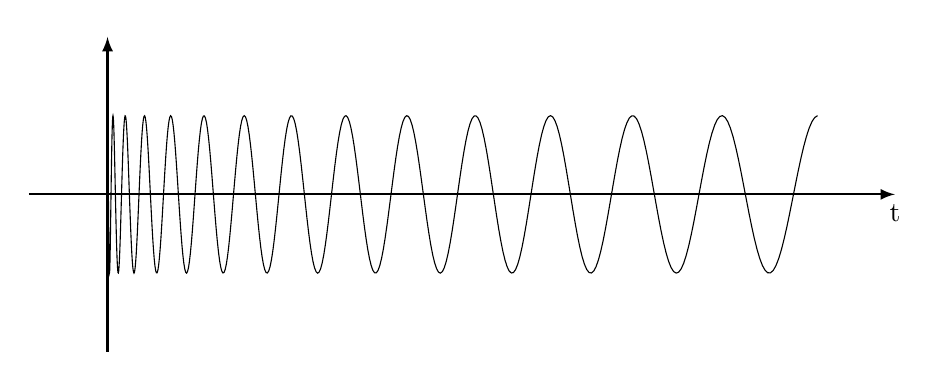
\begin{tikzpicture}
  \draw[thick,-latex] (0,-2) -- (0,2)node[right] {};
  \draw[thick,-latex] (-1,0) -- (10,0)node[below] {t};
  \draw[domain=0.1:9.5,variable=\x,samples=500] plot ({0.10*\x*\x}, {f(\x)});
\end{tikzpicture}
\caption{Down-chirp example\label{fig:downchirp}}
\end{figure}

\subsection{Physical Layer Parameters (PHY)}

This section will cover the major parameters we can tweak in LoRa.
The physical layer parameters are the parameters of the modulations.
Understanding those parameters is important to understand how they modify
the physical property of the modulation and at what cost.
Chapters~\ref{section:radio}~and~\ref{section:tsch} will use these concepts.

\subsubsection{Bandwidth (BW)\label{section:bw}}

Bandwidth is the range of frequencies available during modulation.
LoRa supports three bandwidths in the European sub-GHz ISM band.

\begin{itemize}
    \item 125 kHz
    \item 250 kHz
    \item 500 kHz
\end{itemize}

The BW determines the chip rate and is therefore also expressed in $chips/s$.
 If we are using a $125 kHz$ bandwidth
for our modulation this means $125000 chips / sec$ are transmitted or one chip
each $8 \mu s$.

\begin{equation}
  BW = R_c (chips/s)
\end{equation}

Increasing the BW will then result in an increase in the number of chips sent
per second, directly increasing the quantity of information sent and thus the
data-rate.

\paragraph{}

According to~\cite{semtech:modulationbasics}, increasing the
bandwidth also increases the noise floor which reduces the range of transmission.

\subsubsection{Spreading Factor (SF)}

The spreading factor is a parameter of the LoRa modulation that can range from 7 to 12.
Spreading factors determine two things.

First, the $SF$ value determines the number of bit of information that gets transmitted
per symbols.

\begin{equation}
 \label{eq:sf1}
  SF = \frac{R_b}{R_s}
\end{equation}

Second, $2^{SF}$ equals the number of chips per symbol.

\begin{equation}
 \label{eq:sf2}
  2^{SF} = \frac{chips}{symbols}
\end{equation}

Because the number of chips transmitted per second is depending on the BW,
as we saw in the previous section, increasing the SF results in an increase of
time to transmit a symbol.
We can see the effect of the SF in Fig~\ref{fig:sfcomp},
increasing the SF by one double the time to send a single chirp because it holds
twice as many chips.

We can write the following equation that shows how SF and BW affect the
bit-rate~\cite{semtech:modemdesign} as shown graphically in Fig~\ref{fig:sfcomparaison}
with the comparison table available in Appendix~\ref{table:bitrate}.

\begin{gather}
 \label{eq:bitrate}
  R_{bit} = SF \frac{BW}{2^{SF}}
\end{gather}

% TODO plot graph with equation.

\begin{figure}[H]
  \centering
  \begin{tikzpicture}
  \begin{groupplot}[group style={group size=1 by 2,
      horizontal sep=0pt,
      vertical sep=1cm},
      height=5cm,width=5cm,
  ]
  \nextgroupplot[
    width=0.5\textwidth,
    height=0.5\textwidth,
    axis x line=bottom,
    ymin=0,
    ymax=15000,
    ylabel={$bitrate_{bps}$},
    ylabel near ticks,
    yticklabel style={/pgf/number format/1000 sep=},
    axis y line=left,
    xmin=7,
    xmax=12,
    xlabel={SF},
    xlabel near ticks
  ]
    \addplot[color=red,mark=x] coordinates {
      (7,6836)
      (8,3906)
      (9,2197)
      (10,1220)
      (11,671)
      (12,366)
    };
    \addlegendentry{BW=125kHz}
    \addplot[color=blue] coordinates {
      (7,13671)
      (8,7812)
      (9,4394)
      (10,2441)
      (11,1342)
      (12,732)
    };
    \addlegendentry{BW=250kHz}
  \end{groupplot}
  \end{tikzpicture}
  \caption{SF and BW effect on the bit-rate\label{fig:sfcomparaison}}
\end{figure}


\paragraph{}

Also, a higher SF improves the Signal-to-noise ratio
(SNR) and receiver sensitivity~\cite{semtech:modemdesign}.
This lead to an increase in transmission range.

\paragraph{}

% TODO revoir ca pour être plus explicite

The LoRa modulation uses orthogonal spreading factors to enable concurrent
packet transmission at the same time with different
spreading factors~\cite{semtech:modulationbasics}.

\begin{figure}[H]
\centering
\begin{tikzpicture}[
  arr/.style={help lines,black!70,<->},
]
  \draw[thick,-latex] (0,-2) -- (0,2)node[left] {frequency};
  \draw[thick,-latex] (-1,0) -- (11.5,0)node[below] {time};
  \draw[dashed] (1.5,-2) -- (1.5,2);
  \draw[dashed] (4.5,-2) -- (4.5,2);
  \draw[dashed] (10.5,-2) -- (10.5,2);
  \draw[] (0,-1.8) -- (1.5,1.8);
  \draw[] (1.5,-1.8) -- (4.5,1.8);
  \draw[] (4.5,-1.8) -- (10.5,1.8);

  \draw[arr] (0.1, -2.2) -- node[fill=white] {$SF7$} (1.4, -2.2);
  \draw[arr] (1.6, -2.2) -- node[fill=white] {$SF8$} (4.4, -2.2);
  \draw[arr] (4.6, -2.2) -- node[fill=white] {$SF9$} (10.4, -2.2);
\end{tikzpicture}
\caption{Comparison of the transmission time for a symbol between different SF
  using the same BW\label{fig:sfcomp}}
\end{figure}

\subsubsection{Coding-Rate (CR)}

The CR represents the proportion between information bits and error
correction bits to help with data restoration in case of bit errors
during transmission.

The CR parameter can range from 1 to 4 and stand for the number of correction
bits added every 4 bits of data.
For instance, the parameter CR1 will add 1 correction bit every 4 bits of data
for a total of 5 bits.

Increasing the coding rate will decrease the actual data rate by using
equation~\ref{eq:bitrate} we can know the real data rate of a LoRa transmission.

\begin{equation}
 \label{eq:datarate}
  R_{b} = SF \frac{4}{4 + CR} \frac{BW}{2^{SF}} bits/sec
\end{equation}

The CR introduces more overhead which decreases the data-rate but also
provides more reliable communications.
Table~\ref{table:datarate} available in the appendix for comparison.

% \begin{table}[h!]
% \centering
% \begin{tabular}{@{}ll@{}}
% \hline
% CR & Proportion ($\frac{4}{4 + CR}$) \\ \midrule
% 1                                                & $\frac{4}{5}$\\
% 2                                                & $\frac{4}{6}$\\
% 3                                                & $\frac{4}{7}$\\
% 4                                                & $\frac{4}{8}$\\ \bottomrule
% \end{tabular}
% \caption{Existing Coding Rates\label{table:cr}}
% \end{table}

\subsection{Packet Structure}

LoRa employs two packet formats:
the explicit mode and the implicit mode.
Three parts constitute packets.

\begin{itemize}
  \item Preamble
  \item Optional Header
  \item Data payload
\end{itemize}

\begin{figure}[H]
  \centering
\begin{tikzpicture}[
  timeslot/.style={draw, rectangle, minimum size=1cm},
  description/.style={draw, rectangle, minimum size=1cm},
  arr/.style={help lines,black!70,<->},
]
\begin{scope}[xshift=0cm,yshift=0cm,inner sep=0pt, outer sep=0pt]
  \node (desc0) [description, fit={(0,0) (3.5,2)}, label=center:{Preamble}] {};
  \node (desc1) [description, fit={(3.5,0) (6,2)}, label=center:{Header}] {};
  \node (desc2) [description, fit={(6,0) (7,2)}, label=center:{CRC}] {};
  \node (desc4) [description, fit={(7,0) (11.5,2)}, label=center:{Payload}] {};
  \node (desc5) [description, fit={(11.5,0) (14.5,2)}, label=center:{Payload CRC}] {};
\end{scope}

\draw[arr]
  ([yshift=12pt]desc1.north west) -- node[fill=white] {$CR = \frac{4}{8}$} ([yshift=12pt]{desc2.north east});
\draw[arr]
  ([yshift=-10pt]desc1.south west) -- node[fill=white] {Explicit mode only} ([yshift=-10pt]{desc2.south east});

\draw[arr]
  ([yshift=12pt]desc4.north west) -- node[fill=white] {$CR$} ([yshift=12pt]{desc5.north east});
\end{tikzpicture}
\caption{LoRa Packet Structure\cite{semtech:sx}\label{fig:packetformat}}
\end{figure}

\begin{description}
  \item[Preamble] synchronizes the receiver for the incoming data flow. The
    preamble length is configurable.
  \item[Header] Depends on the packet type explicit or implicit.
  \begin{description}
    \item[Explicit] mode header provides information on the payload.
    \begin{itemize}
      \item Payload length in bytes.
      \item Forward Error Correction code rate.
      \item The presence or not of the payload cyclic redundancy check (CRC).
    \end{itemize}
    \item[Implicit] mode removes the header from the packet. This mode should be
      used when payload, coding rate, and CRC presence are known, and when we want to
      reduce the packet length.
  \end{description}
  \item[Payload] is a variable-length field containing the transmitted data as
    well as an optional CRC.
\end{description}

\subsection{Time on Air (ToA)\label{section:toa}}

The Time on Air is the measure for packet transmission time.
ToA depends on the parameters we introduced previously to count the number of
symbols that constitute each payload.

The following formula defines the duration of each symbol~\ref{eq:tsymlong}.
% Equation~\ref{eq:tsym} is equivalent to the relation~\ref{eq:bw}.

\begin{equation}
  \label{eq:tsymlong}
  T_{sym} = \frac{1}{R_{sym}}
\end{equation}

\begin{equation}
  \label{eq:tsym}
  T_{sym} = \frac{2^{SF}}{BW}
\end{equation}

The ToA is the sum of the time to transmit the packet preamble and the packet
payload.

\begin{equation}
  \label{eq:tpacket}
  T_{packet} = T_{preamble} + T_{payload}
\end{equation}

Equation~\ref{eq:tpreamble} calculates the preamble time. The $n_{preamble}$
or preamble length is programmable.

\begin{equation}
  \label{eq:tpreamble}
  T_{preamble} = (n_{preamble} + 4.25)T_{sym}
\end{equation}

The following equation~\ref{eq:payloadsymnb} gives the number of symbols in the
payload of the packet.
The symbols number depends on the following parameters.

\begin{description}
  \item[PL] The payload length in bytes.
  \item[SF] The spreading factor.
  \item[H] Whether (0) or not (1) the header is enabled.
  \item[DE] Whether (1) or not (0) data rate optimization is enabled.
  \item[CR] The coding rate.
\end{description}

\begin{equation}
  \label{eq:payloadsymnb}
  n_{payload} = 8 + \max(ceil(\frac{8PL - 4SF + 28 + 16 - 20H}{4(SF - 2DE)})(CR + 4),0)
\end{equation}

The payload durations in~\ref{eq:tpayload} give the total packet time on-air
with~\ref{eq:tpacket}.

\begin{equation}
  \label{eq:tpayload}
  T_{payload} = n_{payload} T_{sym}
\end{equation}


\subsection{Channels}

The Things Network~\cite{ttnfrequencyplans} did a summary of the available
channels available depending on the frequency plan of the country the motes are
operating in.

Figure~\ref{fig:channels} presents each LoRaWAN channel available in the
European sub GHz ISM band (863-870 MHz)~\cite{Polonelli_2019}.

\begin{figure}[H]
  \centering
  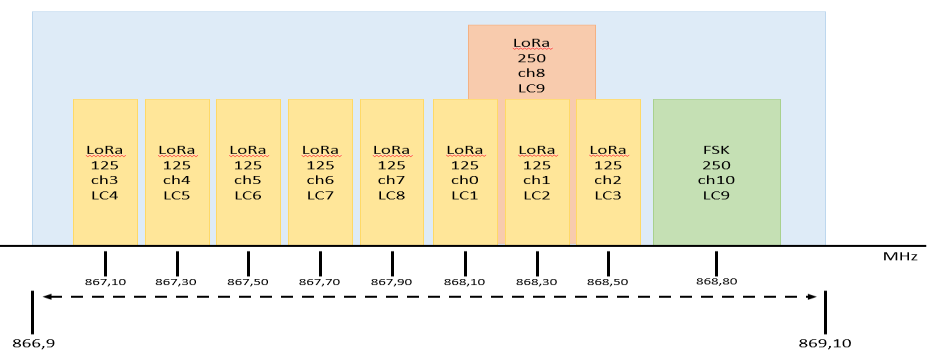
\includegraphics[width=\textwidth]{thesis.tex/chapters/context/fig/channels.png}
  \caption{LoRaWAN Channels in Europe\cite{Polonelli_2019}\label{fig:channels}}
\end{figure}

% TODO explain what is a channel in radio comm and in LoRa and which one we
% will use.

\section{Time-Slotted Channel Hopping (TSCH)}

In traditional star-or-star networks used in LPWAN nodes just wake up
to send their packet to a base station that is always on to listen on all
frequencies and on all spreading factors.

It can be difficult to provide a multi-hop routing protocol that keeps the energy
consumption of your LPWAN as low as possible.
Indeed, now the motes need to wake up at regular moments to be able to serve
as a relay station for their neighbors.
This creates the problem for the mote of knowing \emph{when} to transmit
and on which channel to be able to communicate with their neighbor.
The MAC protocol of the network stack is responsible for those tasks and
is the key to ensure the lowest energy consumption possible.
TSCH is a MAC protocol that can offer a solution for low power and reliable multi-hop routing
because it divides time into time slots that allow certain nodes to sleep while
neighbor is transmitting to a listening node during the same time-slot.

This work, will investigate the feasibility of using TSCH as a MAC protocol for
LoRa-based physical layer networks to achieve a low-power and reliable
multi-hop network.
It is important to understand the subtleties of the functioning of TSCH to
understand the realization presented in this work.
Therefore, TSCH will be presented.

\paragraph{}

% TSCH is a link layer protocol, aiming to achieve reliable communication between
% neighbor nodes and low power operation.
% It takes care of medium access control, duty cycling and synchronisation between nodes.
% Once multi hop is aimed at, routing is needed to guide packet from source to destination.
% It is needed to also study the correct “collaboration” between routing and link layer mechanisms.
%
% TSCH over 802.15.4phy at 2,4Ghz is being  thoroughly studied by the scientific
% community mainly looking at performance parameters such as PDR, power consumption
% and latency and this in function of the choosen scheduling techniques.
% A lot of papers study TSCH under RPL based routing and study schedules that
% adapt to the traffic streams in the RPL tree.
%
% In this work we want to study the feasibility of using TSCH as link layer
% protocol for LoRa-basec physical layer networks.
% Those networks are traditionally star-or-star networks in which nodes wake up
% briefly  to send a packet (and receive the ack)  to a base station that is
% always on to listen on all possible channels.
% In case of “Lora  multi hop networks” consisting of multiple motes based on
% LoRa PHY that help each other to carry packets from source to destination, several issues arise.
% Indeed, now the motes need to wake up at regular moments to be able to serve
% as relay station for their neighbors.
% This creates the problem for the mote of knowing  the when to wake up the
% radio and on which channel to be able to communicate with the neighbor.
% TSCH is a link layer protocol that can (partly?) offer a solution, because it
% allow nodes to sleep in some time slots and to wake up in others to listen while
% a neighbor will be sending in the same slot. The schedule will have arranged
% this “rendez vous”.
% The challenge of porting TSCH from 802.15.4 phy consists in….

TSCH is a Medium Access Control (MAC) layer protocol defined by the IEEE
802.15.4e standard~\cite{rfc7554}.
The design is inherited from WirelessHART and
ISA100.11a~\cite{Duquennoy2017TSCHA6}.
TSCH uses the following principles to achieve low power consumption and
reliability.

\begin{description}
  \item[Time-division multiple access] or (TDMA) by assigning time slots for each
    participant in the network avoiding collisions. The assignment will be done
    by means of the TSCH schedule. This schedule is not part of the TSCH standard.
  \item[Synchronization] time-synchronized nodes syncing their clock with each
    other for being able to keep the notion of \emph{time slot}.
  \item[Multi Channel] for better band usage, less internal interference, and more
    throughput.
  \item[Channel hopping] for combatting external interference
\end{description}

% \subsection{Multiplexing}
%
% To share the same radio communication medium between multiple participants of
% the network, MAC protocol has to implement a sort of channel access method
% based on multiplexing

% TODO Continue and maybe add before TSCH formal intro

\subsection{Time Slots}

Time slots in TSCH are a way to achieve TDMA for the protocol.

A time slot in TSCH is a unit of time to execute the network operations.
The duration of the time slot is not standardized and depends on the physical
layer we are using.
Time slots should be long enough for the longest frame size to be sent
between two nodes, together with an acknowledgement~\cite{rfc7554}.
Every time slot in a TSCH network has the same duration.

For each time slot, a schedule orchestrates what each
node of the network will use his time-slot for: transmit, receive or sleep
(see~\ref{section:tschscheduling} for more details)

Each transmitting or receiving time slot is made of the following parts.

\begin{itemize}
  \item Guard time for time slots synchronization.
  \item The packet transmission or reception.
  \item Acknowledgement reception or transmission.
\end{itemize}

\paragraph{}

A set of time slots that repeat over time is known as a slotframe.
The slotframe length has a direct impact on network capacity.
Figure~\ref{fig:timeslots} represents how time slots and slotframes are
organized together.

\begin{figure}[H]
  \centering

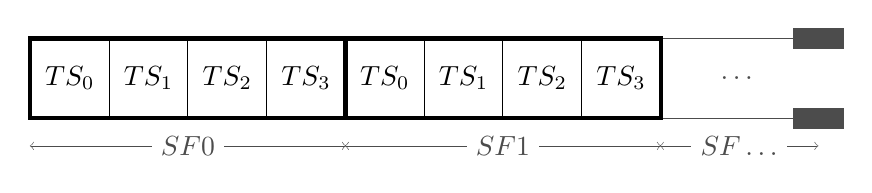
\begin{tikzpicture}[
  timeslot/.style={draw, rectangle, minimum size=1cm},
  arr/.style={help lines,black!70,<->},
]

\foreach [evaluate={\ts=int(mod(\i, 4))}] \i in {0,...,7} {
  \node (ts\i) [timeslot] at (\i, 0) {$TS_{\ts}$};
}
\node (ts8) [minimum height=1cm, minimum width=2cm, black!70] at (8.5, 0) {\ldots};
\draw[help lines, black!70]
  (ts8.north west) -- (ts8.north east) node[fill=white, black!70] {$\ldots$};
\draw[help lines, black!70]
  (ts8.south west) -- (ts8.south east) node[fill=white, black!70] {$\ldots$};

\draw[ultra thick] 
  (ts0.south west) rectangle (ts3.north east)
  (ts4.south west) rectangle (ts7.north east);

\draw[arr]
  ([yshift=-10pt]ts0.south west) -- node[fill=white] {$SF0$} ([yshift=-10pt]{ts3.south east});
\draw[arr]
  ([yshift=-10pt]ts4.south west) -- node[fill=white] {$SF1$} ([yshift=-10pt]{ts7.south east});
\draw[arr]
  ([yshift=-10pt]ts8.south west) -- node[fill=white] {$SF\ldots$} ([yshift=-10pt]{ts8.south east});

\end{tikzpicture}

\caption{Slotframes representation\label{fig:timeslots}}
\end{figure}


\subsection{Absolute Slot Number (ASN)}

The absolute slot number is a shared counter between all the devices that
define the number of time slots elapsed since the start of the
network (see Fig~\ref{fig:asn}).
ASN increases after each time slot and is calculated with \ref{eq:asn} where $k$
is the slotframe offset.

\begin{equation}
  \label{eq:asn}
  ASN = k SF_{len} + TS_{offset}
\end{equation}

\begin{figure}[H]
\centering
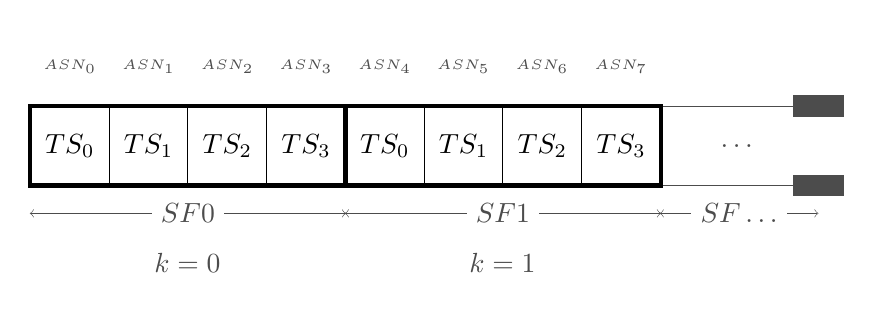
\begin{tikzpicture}[
  asn/.style={black!70, minimum size=1cm},
  timeslot/.style={draw, rectangle, minimum size=1cm},
  arr/.style={help lines,black!70,<->},
  desc/.style={black!70},
]

\foreach \i in {0,...,7} {
  \node (ts\i) [asn] at (\i, 1) {\tiny $ASN_{\i}$};
}
\foreach [evaluate={\ts=int(mod(\i, 4))}] \i in {0,...,7} {
  \node (ts\i) [timeslot] at (\i, 0) {$TS_{\ts}$};
}
\node (ts8) [minimum height=1cm, minimum width=2cm, black!70] at (8.5, 0) {\ldots};
\draw[help lines, black!70]
  (ts8.north west) -- (ts8.north east) node[fill=white, black!70] {$\ldots$};
\draw[help lines, black!70]
  (ts8.south west) -- (ts8.south east) node[fill=white, black!70] {$\ldots$};

\draw[ultra thick] 
  (ts0.south west) rectangle (ts3.north east)
  (ts4.south west) rectangle (ts7.north east);

\draw[arr]
  ([yshift=-10pt]ts0.south west) -- node[fill=white] {$SF0$} ([yshift=-10pt]{ts3.south east});
\draw[arr]
  ([yshift=-10pt]ts4.south west) -- node[fill=white] {$SF1$} ([yshift=-10pt]{ts7.south east});
\draw[arr]
  ([yshift=-10pt]ts8.south west) -- node[fill=white] {$SF\ldots$} ([yshift=-10pt]{ts8.south east});
\node[desc] at
  ([xshift=2cm, yshift=-28pt]ts0.south west) {$k = 0$};
\node[desc] at
  ([xshift=2cm, yshift=-28pt]ts4.south west) {$k = 1$};
\end{tikzpicture}
\caption{Absolute Slot Number\label{fig:asn}}
\end{figure}


\subsection{Channel Hopping}

\emph{Channel Hopping} increases the network capacity with frequency diversity
to mitigate external interferences.
Multiple devices can share time slots to transmit at the same time on different
channels.

Links are the conjunction of a time slot and a channel~\cite{Chen2013PerformanceAO}.

\begin{equation}
  \label{eq:links}
  link = (TimeSlot_{number}, Channel_{offset})
\end{equation}

Multiple links constitute a time slot and devices can transmit on different
links during the same time slot.
This is dependent on the number of channels available.

The channel offset is computed by the transmitter and the receiver with the
function~\ref{eq:channel}. Both nodes know the $ASN$ and the schedule and can
compute the same channel offset~\cite{rfc7554}.

\begin{equation}
  \label{eq:channel}
  Channel_{offset} = (ASN + Scheduled_{offset}) \% Channel_{number}
\end{equation}

If the slotframe length is a prime number, even with the static schedule,
with known channel offset, the time slot will use a different channel every time.
Figure~\ref{fig:channelhopping} shows how scheduled cells in a TSCH network of
four time slots and three channels change channel after each slotframe depending
on the ASN.

\begin{figure}[H]
\centering
\begin{tikzpicture}[
  asn/.style={black!70, minimum size=1cm},
  timeslot/.style={draw, rectangle, minimum size=1cm},
  arr/.style={help lines,black!70,<->},
  desc/.style={black!70},
]

\foreach \i in {0,...,7} {
  \node (asn\i) [asn] at (\i, 4) {\tiny $ASN_{\i}$};
}
\foreach [evaluate={\ts=int(mod(\i, 4))}] \i in {0,...,7} {
  \node (ts3\i) [timeslot] at (\i, 3) {};
}
\foreach [evaluate={\ts=int(mod(\i, 4))}] \i in {0,...,7} {
  \node (ts2\i) [timeslot] at (\i, 2) {};
}
\foreach [evaluate={\ts=int(mod(\i, 4))}] \i in {0,...,7} {
  \node (ts1\i) [timeslot] at (\i, 1) {};
}
\foreach [evaluate={\ts=int(mod(\i, 4))}] \i in {0,...,7} {
  \node (ts\i) [asn] at (\i, 0) {$TS_{\ts}$};
}
% \node (ts8) [minimum height=1cm, minimum width=2cm, black!70] at (8.5, 0) {\ldots};
% \draw[help lines, black!70]
%   (ts8.north west) -- (ts8.north east) node[fill=white, black!70] {$\ldots$};
% \draw[help lines, black!70]
%   (ts8.south west) -- (ts8.south east) node[fill=white, black!70] {$\ldots$};

\node (choff3) [black!70] at (-1.5, 3) {$Ch_{off} 2$};
\node (choff2) [black!70] at (-1.5, 2) {$Ch_{off} 1$};
\node (choff1) [black!70] at (-1.5, 1) {$Ch_{off} 0$};

\begin{scope}[on background layer]
\fill[blue!50] (ts10.south west) rectangle (ts10.north east);
\fill[blue!50] (ts24.south west) rectangle (ts24.north east);

\fill[orange!50] (ts30.south west) rectangle (ts30.north east);
\fill[orange!50] (ts14.south west) rectangle (ts14.north east);

\fill[green!50] (ts22.south west) rectangle (ts22.north east);
\fill[green!50] (ts36.south west) rectangle (ts36.north east);
\end{scope}

\draw[ultra thick] 
  (ts10.south west) rectangle (ts33.north east)
  (ts14.south west) rectangle (ts37.north east);

\draw[arr]
  ([yshift=-10pt]ts0.south west) -- node[fill=white] {$SF0$} ([yshift=-10pt]{ts3.south east});
\draw[arr]
  ([yshift=-10pt]ts4.south west) -- node[fill=white] {$SF1$} ([yshift=-10pt]{ts7.south east});
\draw[arr]
  ([yshift=-10pt]ts8.south west) -- node[fill=white] {$SF\ldots$} ([yshift=-10pt]{ts8.south east});
\node[desc] at
  ([xshift=2cm, yshift=-28pt]ts0.south west) {$k = 0$};
\node[desc] at
  ([xshift=2cm, yshift=-28pt]ts4.south west) {$k = 1$};
\end{tikzpicture}
\caption{Two slotframes with scheduled cells changing channel between slotframes\label{fig:channelhopping}}
\end{figure}


\subsection{Scheduling\label{section:tschscheduling}}

The TSCH schedule tells each node what to do during a time slot and defines the
following parameters for each time slot.

\begin{itemize}
  \item Receive or transmit or sleep.
  \item The channel offset in case of transmit or receive.
  \item Address of the node or nodes to communicate with.
\end{itemize}

To ensure the synchronization of the slots, each transmission is taken as an opportunity
for the neighbor to resynchronize its clock.
Synchronization is important to mitigate each node's internal clock drift.

Time source (or coordinator) nodes send Enhanced Beacon (EB) packets to synchronize the receiving
nodes of the network. When nodes do not resynchronize for a long period
a Keep-Alive (KA) is sent and used to adjust the drift at synchronization.

Figure~\ref{fig:sync} represents the clock drift that can occur between two
distant time slots.
As we can see the receiver will know the drift based at the moment he receives
the data and then adjusts its time slot length to finish earlier.

\begin{figure}[H]
  \centering
  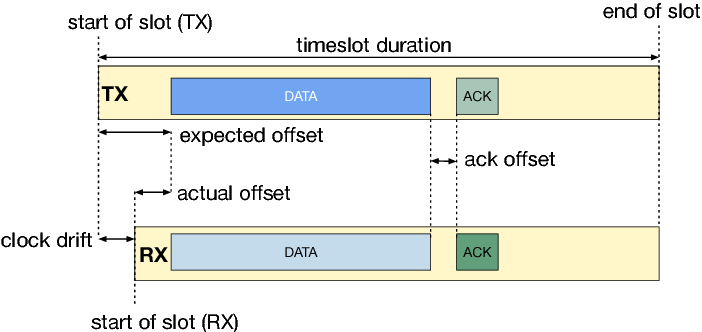
\includegraphics[width=\textwidth]{thesis.tex/chapters/context/fig/sync.png}
  \caption{Synchronization in a TSCH time slot\cite{TELESHERMETO201784}\label{fig:sync}}
\end{figure}

\section{Routing}

Adapting TSCH is not the only step to achieve low-power
multi-hop routing.
An appropriate routing protocol is needed to guide packets from source to destination.
We can use already existing low power multi-hop routing protocols that do not need
to be re-implemented.

I will use the RPL routing protocols and the Orchestra scheduler for TSCH in
Chapter~\ref{section:tsch} to test that the adaptation of TSCH I made worked
with LoRa.

\paragraph{}

I will introduce in this section the protocol I used: RPL and Orchestra.
This section is not meant to be an in-depth explanation of the protocols.
Giving such details would be out of the scope of my work as I do not modify any
of the components of those protocols.

\subsection{Routing Protocol for Low-Power and Lossy Networks (RPL)}

RPL is a routing protocol for constrained device networks.
RPL is designed to work on networks with high data loss rates, low data rates, and
instability~\cite{rfc6550}.

The routing in RPL is based on Destination Oriented Directed Acyclic Graphs (DODAG).
All the nodes of the DODAG route toward the \emph{root} node.
If the root node is connected to the internet it can be used as a \emph{border
router}.
RPL gives each node a rank based on the distance from the root node.
The distance is calculated with an \emph{objective function}.
The routing between nodes in RPL is based on sending packets up to a smaller
ranked parent until it reaches a common ancestor and then sending the packet down
to the destination~\cite{duquennoy2015}.

\subsection{Orchestra}

Orchestra is a scheduler that works on top of TSCH+RPL
networks where each node autonomously computes its schedule without the
need of a centralised scheduler~\cite{duquennoy2015}.
Each node maintains its schedule and keeps track of its neighbors solely
on the network information from RPL.
Orchestra maintains different slotframes for these different network operations

\begin{itemize}
  \item Application data
  \item RPL control traffic
  \item TSCH beacon
\end{itemize}

Using mutually prime slotframe lengths
makes sure they cycle independently and avoids persisting overlap.
For the regular traffic between nodes, organizing a schedule by computing time
and channel offset using the sender and receiver
identification as parameters, Orchestra can achieve a very low level of
collisions between concurrent data streams~\cite{duquennoy2015}.

\section{Contiki OS}

Embedded operating systems help developers in the process of writing programs
for embedded systems.
As a starting point for my work, the Contiki-NG lightweight operating system (OS)
that contains a full-fledged IPv6 protocol stack for short range 802.15.4 Phy
TSCH based networks, is taken.
Re-implementing a whole network stack is out of the scope of this project and
re-using each network layer available in Contiki to conduct my testing will
speed up my development.
Only the existing implementation of TSCH will be judiciously modified in
chapter~\ref{section:tsch} and a new radio driver will be added to
the OS in chapter~\ref{section:radio}.

\paragraph{}

Contiki is a free and open-source Real-Time operating system (OS) specifically made
for IoT applications.
Contiki uses protothreads, a programming abstraction which Contiki is
built around.
They allow developers to write event-driven programs with little memory overhead and
reduce the complexity of embedded programs that used to be written
like state machines~\cite{10.1145/1182807.1182811}.

The Contiki OS project has been unmaintained since 2017 but its
successor named Contiki-NG was created as a fork by the same developers since.
That fork has been the basis for a lot of LPWAN experimentation, for example
with the development of the 6TiSCH stack for the OS~\cite{Duquennoy2017TSCHA6}.

\subsection{NETSTACK}

Contiki's Network Protocol stack, also known as \lstinline{NETSTACK}, is a
feature of the OS.
It allows developers to define parts of the network stack we are using in a Contiki
project (Fig~\ref{fig:netstack}).

NETSTACK implementation allows Contiki to communicate between layers without
knowing the specific implementation of the layer.
Developers must define the following variables to change the network stack
in a Contiki project.

\begin{itemize}
  \item \lstinline{NETSTACK_NETWORK}
  \item \lstinline{NETSTACK_ROUTING}
  \item \lstinline{NETSTACK_MAC}
  \item \lstinline{NETSTACK_RADIO}
\end{itemize}

Each layer of the NETSTACK has its own set of functions available.
NETSTACK will allow us to define our new radio driver in
chapter~\ref{section:radio} under the \lstinline{NETSTACK_RADIO}
abstraction layer that prevents us to redefine every part of the upper
\lstinline{NETSTACK_MAC} layer.

\begin{figure}[H]
\centering
  \begin{tikzpicture}[->,>=stealth',shorten >=1pt,auto,node distance=1.4cm]

  \tikzstyle{comment}=[
    right=2pt,
    font=\small,
    fill=white,
    text=black,
    draw=black,
  ]

  \tikzstyle{every state}=[rectangle,thick,
    draw=black,fill=gray!20,text=black,
    minimum width= 6cm,
    minimum height= 1.20cm
  ]

  \tikzstyle{smallstate}=[rectangle,thick,
    draw=black,fill=gray!10,text=black,
    minimum width= 4cm,
    minimum height= 1.20cm
  ]

  \node[smallstate]         (A)                    {Network Layer};
  \node[smallstate]         (B) [below of=A]       {Routing};
\begin{scope}[on background layer]
  \node[state, fit=(A)(B)] (AB)                 {};
\end{scope}
  \node[state,below=1cm]         (C) [below of=AB]       {MAC Layer};
  \node[state]         (D) [below of=C]       {Physical Layer};

  \node[comment]       at (AB.north west) {Network Layer};
  % \node[comment]       at (C.north west) {MAC Layer};
  % \node[comment]       at (D.north west) {Physical Layer};
  % \path (A) edge [bend right]    node {     } (B)
  %           edge [bend left]     node {     } (C)
  %       (B) edge [bend left]     node {     } (C)
  %           edge                 node {     } (D)
  %       (C) edge [bend left]     node {     } (A)
  %       (D) edge [bend right=85] node {     } (A);
\end{tikzpicture}
\caption{The Contiki's Network Protocol Stack\label{fig:netstack}}
\end{figure}


\section{Related work}

This is not the first attempt to bring multi-hop communication to LoRa.
Multi-hop communication solves the following issues inherent to the original
LoRaWAN architecture.

\begin{itemize}
  \item There is no coordination between nodes and most of them transmit on the
    same channel and same SF, this leads to collision and low packet delivery
    rate (PDR) on dense networks. On collision, the packet is retransmitted
    which implies a higher energy consumption for the mote.
  \item Nodes on the edge of the gateway coverage fail most of the time to
    complete their transmission to the gateway. Edge nodes are using the
    highest SF factor to achieve the highest range but it also has
    the longest time on air and the worst energy performance.
    The SF in conjunction with the retransmission leads to bad energy performance.
  \item There are some use cases where gateways are just impossible to install
    and using motes to relay messages to gateways is needed.
\end{itemize}

This section will give a state of the art of the research on
multi-hop routing in LoRa with the aim to address some of the issue
aforementioned.

\paragraph{}

Work to port TSCH and the 6LoWPAN stack to a new radio protocol has already
been done in~\cite{uwbtsch} for the Ultra-Wide Band (UWB).

\paragraph{UWB-TSCH}

Charlier M. in~\cite{uwbtsch} explores the requirements to adapt TSCH for the UWB.
Similarl to LoRa, UWB does not allow CCA and thus can not use CSMA for its
communications.
His work shows what it takes to adapt TSCH for another radio layer.
It is also an evaluation of the performance of TSCH outside of 802.15.4.

\paragraph{}

The respective authors of~\cite{DIAS2018424, 8856256}, look at ways to extend
the current LoRaWAN MAC protocol to allow multi-hop communications.

\paragraph{Multihop LoRaWAN Extension} Dias J., Grilo A. in \cite{DIAS2018424}
design a routing protocol that can interoperate with LoRaWAN gateways while
using multi-hop communications for nodes out of the range of the gateway.
The extension uses beacons to achieve time synchronization to achieve low power
multi-hopping.
No channel hopping is used though, unique channel congestion is already an issue
in LoRaWAN and this work makes the matter worst.
This work focus on resolving the range issue of the bordering nodes.

% \subsection{RS LoRa}
% [18] in roald similar to lorawan extension
% \subsection{Listen before talk LoRa}
% [17] in roald work

\paragraph{}

Studies on creating a new MAC protocol for multi-hop LoRa communications in a linear
network has been done in~\cite{Abrardo_2019,duong2018}.

\paragraph{Linear Multihop LoRa}

Abrardo A. and Pozzebon A.~\cite{Abrardo_2019} studied the deployment of a
large scale LoRa network to monitor the underground medieval aqueducts of the city center
of Sienna, the \emph{Bottini}.

Because of the large deployment cost induced by the large tunnels, the negative
aesthetic impact of a wired network, and the risk of flooding,
the usual LoRaWAN architecture using gateways was impossible and made the author
opt for a battery-operated LoRa network.
To solve this issue, they propose a multi-hop routing solution for Linear Sensor
Network (LSN) by developing their own MAC protocol tailored for their scenario.
This custom protocol is built around assigning time slots for each node with
a common schedule for adjacent nodes.
This allows neighbors to synchronize their clock and broadcast messages to
both ends of the aqueducts.

While their solution solves their particular problem all the schedules are hard-coded,
there is no discovery mechanism in the protocol.
This solution scales badly and cannot suit a non-linear network.

% Their solution allowed the connection of the Bottini

\paragraph{Multi-Hop Linear Network Based on LoRa}

Duong T. in~\cite{duong2018} proposes a multi-hop protocol for LoRa linear
networks.
His network is made of two periods. The first is the network initialization to
verify the gateway is reachable and synchronizes the nodes to make them join the
data operation period.
Each node transmits in a different time slot to their parent node, each hop adds
their information to the packet they are relaying until the gateway is
reached.
The clock drift is mitigated by synchronizing on the preamble but the receiver
does not acknowledge the reception of the packet, making the network unreliable
and sensible to interference and collision since it is running on a
single channel and SF.
Also, the initialization period is unique, which makes the network impossible to
scale once it is running.

\paragraph{}

The next studies look at ways to create a fully functioning multi-hop network
using LoRa without depending on LoRaWAN specifications.

\paragraph{LoRaBlink}

Bor M., Vidler J., Roedig Utz. in \cite{lorablink} propose the LoRaBlink
protocol, designed to support reliable and energy efficient multi-hop
communication.

Each node of the network remains in listening mode until a beacon is received.
Beacons are used for time synchronization of the time slots.
Each node transmits packets to their parent node that relays it to the gateway.
Because the protocol is designed to work on a single channel and
there is no scheduling of when a node can transmit, packet collision often occur
which, as the number of device increase in the network, affects a lot the
performance of the network.

Also, using a single SF, BW, and channel. It decreases the overall throughput
of the network and makes it highly sensitive to interference.

\paragraph{RPL+LoRa MAC Protocol}

B. Sartori, S. Thielemans, M. Bezunartea, A. Braeken, and K. Steenhaut~\cite{8115756}
from the SmartNet research group of VUB, adapted RPL
to enable multihop communications on top of LoRa.
The work presents the modifications of the objective function to take into
account the SF when computing the best routes as well as the creation of a MAC
protocol, \emph{RLMAC} to manage time slots.
This work describes a solution for a network of nodes to discover each other.
It uses a router sending packets on different spreading factors while the joining
node listens on the spreading factors by starting by the lowest, this way it
picks the fastest spreading factor available.
The custom MAC protocol, \emph{RLMAC}, built in this paper to allow multi-hop
routing with LoRa manages time slots between nodes and allows PHY settings
tuning depending on the links.

% But the discovery made it non power efficient

The protocol proposed focused on having total lowest time on air on a path from
mote to sink with LoRa
communications for increasing the packet delivery rate (PDR).
Reducing the power consumption was not a concern in this paper.

\paragraph{TSCH-over-LoRa}

Haubro M., Orfanadis C., Oikonomou G., and Fafoutis X.~\cite{tschoverlora}
have recently published a work studying the feasibility of porting TSCH to LoRa
in Contiki OS using the SX1272 radio module.

The authors have shown it was possible to adapt TSCH for LoRa by testing their
implementation with a variety of routing protocols and applications.
Their implementation works on a single SF at a time and tested it using
SF7 and SF10.

To demonstrate the resilience of TSCH to interference even with LoRa, the
authors made a radio jammer that transmits on different channels. Their
experimentation showed no packets got lost when using channel hopping with
LoRa.

\section{Conclusion}

The typical LPWAN network architecture is based on a star-of-star topology
with gateways that listen for incoming messages on every possible channel.
This design keeps the power consumption of the motes as low as possible
but, as the network grows, lack of coordination between the participant to avoid
collisions and can suffer from communication range issues.

A LoRa multi-hop network consists of motes based on the LoRa radio protocol
that helps each other to carry packets from source to destination.
The concern building a low-power multi-hop network is to keep
the radio turned-on as low as possible while still being able to relay
messages between neighbors by turning-on the radio during a synchronized time frame.
A mote can only send/listen on one channel at the same time.
This creates the problem for the mote of knowing when to wake up the radio and
on which channel to be able to communicate with the neighbor.
TSCH is a MAC protocol that
can offer a low-power and reliable solution because it synchronizes nodes
to sleep in time slots to achieve the lowest power consumption possible for the
radios and use channel hopping to achieve frequency diversity and thus be
more reliable and less subject to interference.
To achieve multi-hop, routing is still needed to guide packet from source
to destination but already existing protocols like RPL that have been studied
in conjunction with TSCH could be used.
As a starting point, Contiki OS will be used as it bundle with a
implementation of TSCH and RPL and a full-fledged IPv6 protocol stack.

There has already been an attempt to create LoRa multi-hop network in the
literature the issue is most of them designed their routing and MAC protocol
rather than starting from the existing implementation.
This lead to protocols that have two main issues.
First, they don't take into account the frequency diversity by
not including any channel-hopping mechanisms, making the protocols subject to
collisions as well as limited data rate as two nodes cannot transmit at the same time.
Second, they often do not include any joining procedure
for new nodes to join the running network which prevents the network from growing.
